% !TeX root = main.tex
\lecture{4}{Thu 09 Oct 2025 13:00}{Waves at Boundaries}

\section*{Recap}

We previously derived:
\[
    v = \sqrt{\frac{T}{\mu}}
\]

And we also have:
\[
    v = \frac{\omega}{k}
\]

The former is useful explictly for a wave travelling over a string, while the latter is applicable to the movement of any wave. On a string, a higher tension yields a higher restoring force and therefore a higher speed, while a higher mass per unit length gives a higher mass for some arbitrary length of string, therefore a lower acceleration and lower speed.

\section*{A Quick Interlude}
The speed of a mechanical wave has the general form:
\[
    v = \sqrt{\frac{\text{Restoring force returning to equilibrium}}{\text{Inertia resisting return to equilibrium}}}
\]

\section*{Reflection}
When a wave hits a fixed boundary, it is reflected and inverted. Lets consider a case where a string is fixed on the LHS and is reflected back:
\begin{figure}[H]
    \centering
    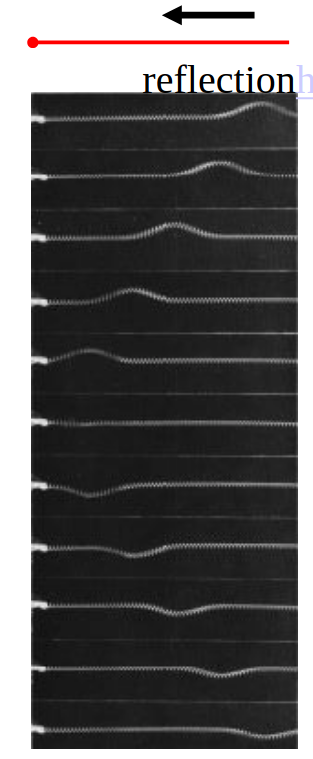
\includegraphics{figures/lec04-02.png}
\end{figure}

\begin{figure}[H]
    \centering
    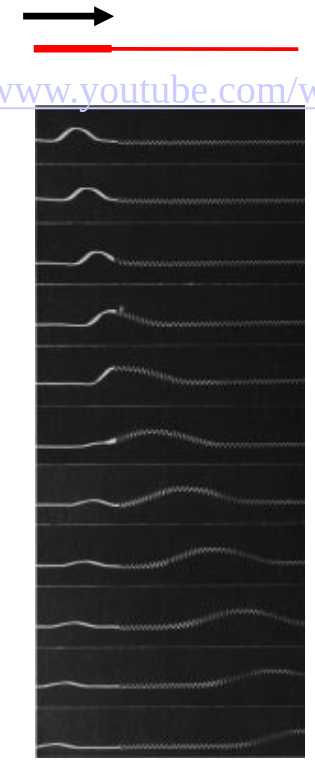
\includegraphics{figures/lec04-03.png}
     \caption{Or with two strings, going from thick to thin:
}
\end{figure}

\begin{figure}[H]
    \centering
    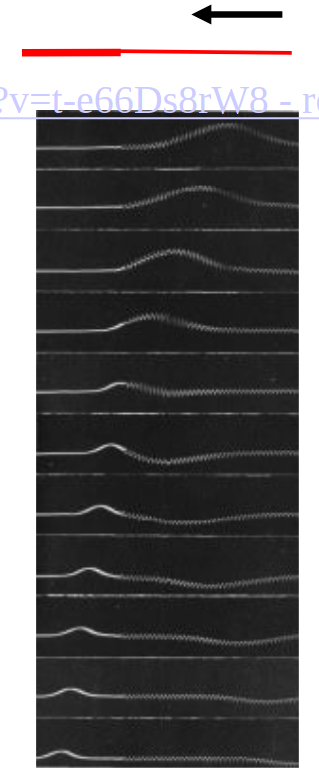
\includegraphics{figures/lec04-04.png}
     \caption{Or from thin to thick.}
\end{figure}

\section*{Waves Interacting at Boundaries}
Say we have two pieces of string connected to each other, one thin string with mass per unit length $\mu_1$ and a thicker string with $\mu_2$ (both under the same tension, $T$). If a wave pulse is passed along from the thin string to the thicker string, whath happens at the point of connection, $P$?
\begin{figure}[H]
    \centering
    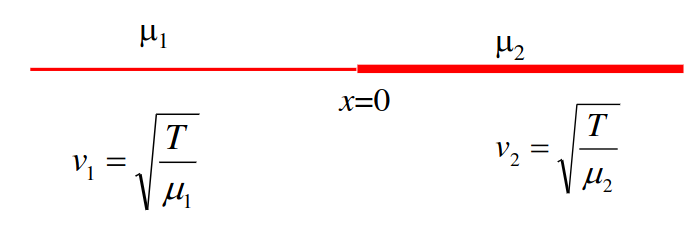
\includegraphics[width=0.75\textwidth]{figures/lec04-01.png}
     \caption{The two connected strings.}
\end{figure}

Consider a travelling wave coming from the left:
\[
    y_1 = A \cos(k_1 x - \omega_1 t)
\]

\[
    y_2 = B \cos(k_2 x - \omega_2 t)
\]

At the point of connection, we'll define this as $x = 0$. Here (as the string is not broken, so it must be connected):
\begin{equation}
    y_1 = y_2
\end{equation}

Also, force is finite, therefore curvature must be finite (as force is proportional to curvature). Therefore we cannot have any discontinuities in curvature.
\begin{equation}
    \frac{\partial y_1}{\partial x_1} = \frac{\partial y_2}{\partial x_2}
\end{equation}

Disregarding non-linear effects, so assuming that the frequency with which the waves travel down the string is the same for both parts of the string, $\omega_1 = \omega_2 = \omega$.

From (1) and noting $x = 0$:
\begin{equation}
    A \cos(-\omega t) = B \cos(\omega t)
\end{equation}

And from (2) with the same note:
\begin{equation}
    -k_1 A \sin -\omega t = -k_2 B \sin -\omega t
\end{equation}

However this suggests that $A = B = 0$. This is technically a solution, but not really - it doesn't represent an actual wave (just two flat lines with no amplitude ever)

\subsection*{Including Reflection}
The previous case did not work as we disregarded reflection at the wave boundary, $P$. Lets add an extra wave (the C term) to represent the reflection back into the light string:
\[
    y_1 = A \cos(k_1 x - \omega t) + C \cos(k_1 x + \omega t) = B \cos(k_2 x - \omega t)
\]

From y1 = y2 at x = 0 we get:
\[
        y_1 = A \cos(- \omega t) + C \cos( -\omega t) = B \cos( - \omega t)
\]
So: $A+C = B$
 
From (2) we get:
\[
    -k_1 A \sin(- \omega t) - k_1 C \sin(\omega t) = -k_2 B \sin(-\omega t)
\]

Which has solutions:
\[
    B = \frac{2k_1}{k_1 + k_2} A
\]
\[
    C = \frac{k_1 - k_2}{k_1 + k_2}A
\]

We have the incident wave:
\[
    y_1 = Acos(k_1 x - \omega t)    
\]

The transmitted wave:
\[
    y_2 = B \cos(k_2 x - \omega t) = \frac{2k_1}{k_1 + k_2} A \cos(k_2 x - \omega t)
\]

And lastly the reflected wave:
\[
    y_3 = C \cos(k_1 x + \omega t) = \frac{k_1 - k_2}{k_1 + k_2} A \cos(k_1 x - \omega t)
\]


We note:

$k_1$ is the wave number in the medium where the incident wave comes from.

$k_2$ is the wave number in the medium where the transmitted wave goes into.

\subsection*{Example}
If the wave comes in from the left, then $\mu_2 > \mu_1$ per example diagram, then $k_2 > k_1$, and $C$ is negative.

Note that if the single pulse as a postive y amplitude, then the transmitted pulse in the heavier string will also have a positive y amplitude, but will have a smaller magnitude. The reflected wave will have a negative y-amplitude as the reflection inverts it.

If the wave comes from the right (from thick to thin), then $\mu_1 > \mu_2$, $k_1 > k_2$ and C is positive.